\documentclass{standalone}
\usepackage{tikz}
\usetikzlibrary{shapes.geometric,decorations.markings,arrows}

\newcommand\R{2.5em}
\tikzset{
    buffer/.style={
        draw,
        %% shape border rotate=180,
        regular polygon,
        regular polygon sides=3,
        node distance=3cm,
        minimum height=6em
    }
}

\begin{document}
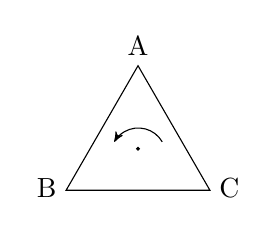
\begin{tikzpicture}
  \node[buffer]{};
  % кружок в центре треугольника
  \draw[fill,radius=0.5pt] (0,0) circle {};
  \node at (-3.3em, -0.5) {B};
  \node at (0, 3.7em) {A};
  \node at (3.3em, -0.5) {C};
  \draw[-stealth'] (0.35*\R, 0.1*\R) arc (-330:-210:{0.4*\R});
\end{tikzpicture}
\end{document}
